 																							                               	%---Orsay---%
%%%%%%%%%%%%%%%%%%%%%%%%%%%%%%%%%%%%%%%%%%%%%%%%%%%%%%%%%%%%%%%%%%%%%%%%%%%%%%%%%%%%%%%%%%%%%%%%%%

\documentclass[a4paper,11pt]{article}

%---Packages utilisés
\usepackage[utf8]{inputenc}
\usepackage[T1]{fontenc}
\usepackage[frenchb]{babel}
\usepackage{indentfirst}
\usepackage[]{graphicx}
\usepackage{amsmath}
\usepackage{ccaption}
\usepackage{vmargin}
\usepackage{textcomp}
\usepackage{fancyhdr}
%\usepackage[avantgarde]{quotchap}
\usepackage[Lenny]{fncychap}
\usepackage{cite}
\usepackage{color}

\fancypagestyle{plain}{
\fancyhead[]{}
\fancyfoot[R]{\thepage}
\renewcommand{\headrulewidth}{0pt}}

%---Nouvelles commandes
\newcommand{\cyrce}{\textsc{Cyrcé}}
\newcommand{\Root}{\textsc{Root}}
\renewcommand{\baselinestretch}{1.2}
\newcommand{\alp}{$\alpha$}
\newcommand{\Asta}{$^{211}$At}
\newcommand{\AstaIso}{$^{210}$At}

%\renewcommand{\chaptermark}[1]{%
% \markboth{\thechapter . \ #1}{}}

%---Mise en page
\setlength{\parindent}{2ex}
%\pagestyle{fancy}

%---Début du document
\begin{document}

%---Marges du document
\setmarginsrb{3.5cm}{1.5cm}{1.5cm}{2cm}{2ex}{3ex}{2ex}{5ex}
%1 est la marge gauche
%2 est la marge en haut
%3 est la marge droite 
%4 est la marge en bas
%5 fixe la hauteur de l'etête
%6 fixe la distance entre l'entte et le texte
%7 fixe la hauteur du pied de page
%8 fixe la distance entre le texte et le pied de page
%
%\chapterstyle{veelo}
%\renewcommand{\sectionmark}[1]{\markright{\thesection\ #1}}
\lhead[]{}
\fancyfoot[C]{}
\fancyfoot[R]{\thepage}

%%%%%%%%%%%%%%%%
\begin{center}
\subsection*{Analyse des données issues des irradiations sur Kinétron}
\end{center}

\subsection*{Protocole des mesures}
La nouvelle chambre Exocet équipée d'une cuillère de détection de 1~cm$^2$ et d'un gap de 800~microns  est placée en sortie direct du Kinétron.
Le PM est posé derrière une protection en plomb pour diminuer l'intensité du rayonnement diffusé.
Un collimateur propre au Kinétron et servant de mesure est également utilisé.
Chacun de ces trois signaux est redirigé vers l'oscilloscope où notamment le PM pourra servir de \emph{trigger} de déclenchement.

En plus de celui de \emph{trigger}, le rôle du PM est de servir de référence vers les hautes intensités pour lesquelles il reste, modulant sa tension, linéaire.

Les tensions propres à la chambre et au PM peuvent être modulées.

Le but de ces manips était de mesurer la contribution uniquement électronique du signal.

\newpage
\subsection*{Rappel de l'ensemble des irradiations}
Pour toutes les mesures, la fréquence de pulse est de 10~Hz et les signaux sont labellisés de la sorte :
\begin{itemize}
\item C1 $\rightarrow$ chambre,
\item C2 $\rightarrow$ PM,
\item C3 $\rightarrow$ collimateur.
\end{itemize} 
\`A chaque fois 100 pulses sont envoyés.
Pour cette première série, leur largeur est fixe à 1~$\mu s$.
\begin{center}
\begin{tabular}{rlcccc}
\multicolumn{3}{c}{Fichier}&\multicolumn{3}{c}{Tensions (V)}\\
Pré.&Num.&Ind.&Grille&PM&Chambre\\
\hline
\hline
manip&1&0-99&100&1100&500\\
&2&0-99&\textcolor{red}{120}&1100&500\\
&3&0-99&\textcolor{red}{140}&1100&500\\
&3-1&0-99&140&\textcolor{red}{1050}&500\\
&3-2&0-99&140&\textcolor{red}{1000}&500\\
&3-3&0-99&140&\textcolor{red}{950}&500\\
&4&0-99&\textcolor{red}{160}&950&500\\
&4-1&0-99&160&\textcolor{red}{900}&500\\
\multicolumn{6}{c}{Adaptation faraday (un bouchon 50~$\Omega$ retiré)}\\
&4-2&0-99&160&900&500\\
&5&0-99&\textcolor{red}{180}&900&500\\
&5-1&0-99&180&\textcolor{red}{850}&500\\
&6&26-125&\textcolor{red}{200}&850&500\\
&7&0-99&\textcolor{red}{220}&850&500\\
&7-1&0-99&220&850&\textcolor{red}{100}\\
&7-2&0-99&220&850&\textcolor{red}{50}\\
&7-3&0-99&220&850&\textcolor{red}{200}\\
&7-4&0-99&220&850&\textcolor{red}{300}\\
&7-5&0-99&220&850&\textcolor{red}{400}\\
&7-6&0-99&220&850&\textcolor{red}{600}\\
&7-7&0-99&220&850&\textcolor{red}{700}\\
&8&0-99&220&\textcolor{red}{800}&700\\
&9&0-99&\textcolor{red}{240}&800&700\\
&10&0-99&\textcolor{red}{260}&800&700\\
&10-1&2-101&260&\textcolor{red}{750}&700\\
&11&0-99&\textcolor{red}{280}&750&700\\
&12&0-99&\textcolor{red}{300}&750&700\\
\hline
\end{tabular}
\end{center}

\newpage
Pour cette seconde série, les tensions du PM et de la grille sont fixes, respectivement à 850~V et 300~V.
\begin{center}
\begin{tabular}{rlccc}
\multicolumn{3}{c}{Fichier}&Tension&Largeur\\
Pré.&Num.&Ind.&chambre (V)&pulse ($\mu s$)\\
\hline
\hline
manip\_largeur&1&0-99&700&0.1\\
&1-2&0-99&700&0.1\\
&2&0-99&700&\textcolor{red}{0.3}\\
&3&0-99&700&\textcolor{red}{0.5}\\
&4&0-99&700&\textcolor{red}{0.8}\\
&5&0-99&700&\textcolor{red}{1.2}\\
&6&0-99&700&\textcolor{red}{1.4}\\
&7&0-99&700&\textcolor{red}{1.8}\\
&8&0-99&700&\textcolor{red}{2.2}\\
&8-1&0-99&\textcolor{red}{300}&2.2\\
&8-3&0-99&\textcolor{red}{500}&2.2\\
&8-4&0-99&\textcolor{red}{900}&2.2\\
&8-5&0-99&\textcolor{red}{1000}&2.2\\
&8-6&0-99&\textcolor{red}{1200}&2.2\\
\hline
\end{tabular}
\end{center}

\subsection*{Mesures sur l'oscilloscope}

Les figures \ref{fig:manip1_1} présentent l'affichage sur l'oscilloscope pour un pulse de faisceau. 
Le signal rouge du PM fait donc office de \emph{trigger} et permet ainsi le déclenchement de l'acquisition.
Nous pouvons observer, notamment sur le signal du collimateur, jaune, les perturbations dues à la HF en amont.
Les mesures de piédestaux seront ainsi effectuées entre -4~$\mu$s et -2~$\mu$s.

Les signaux issus des chambres ayant des amplitudes bien moindres sont à peine visibles sur ces deux images.
Les figures \ref{fig:manip1_2} présentent elles ces signaux isolés.
Nous y distinguons également en rouge, le calcul de la ligne de base permettant la soustraction des contributions ioniques aux signaux.
Bien que plus lents, les ions se déplacent tout de même durant le temps du pulse, générant ainsi un signal que nous pouvons observer par le décalage en hauteur des piédestaux avant et après le signal électronique.
Pour retirer cette contribution, l'aire d'un simple triangle est soustraite à l'intégrale du signal. 
\begin{figure}[h]
\begin{center}
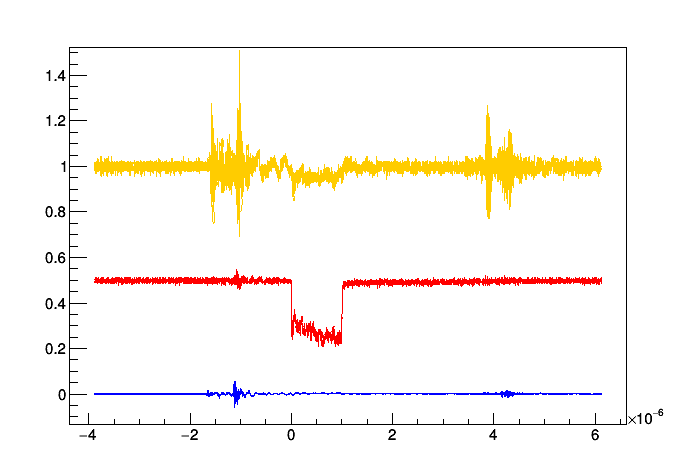
\includegraphics[width=\linewidth]{manip1_1.png} 
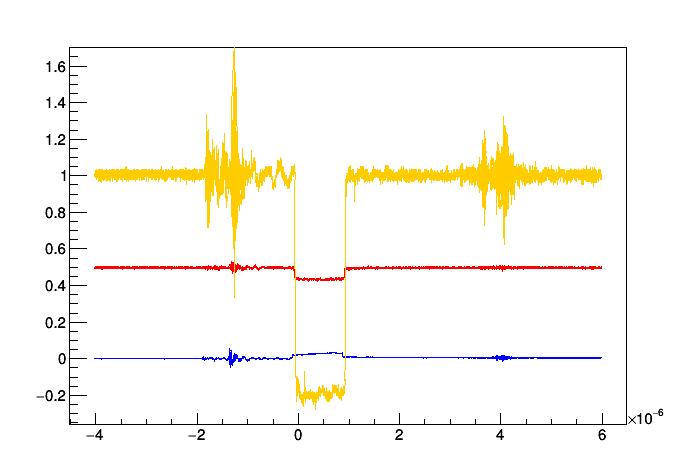
\includegraphics[width=\linewidth]{manip12_2.png} 
\caption{\label{fig:manip1_1}\footnotesize{Affichage sur l'oscilloscope pour le premier pulse de la première mesure, en haut, et pour le premier pulse de la dernière mesure, en bas. En jaune nous avons le signal issu du collimateur, en rouge celui du PM et en bleu celui de la chambre, les deux premiers sont décalés en ordonnée pour favoriser la lecture. L'axe des abscisses est exprimé en secondes.}}
\end{center}
\end{figure}

\begin{figure}[h]
\begin{center}
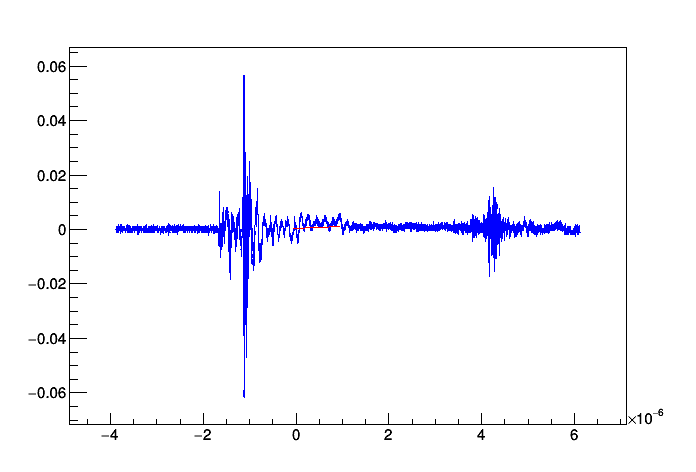
\includegraphics[width=\linewidth]{manip1_1_chambre.png} 
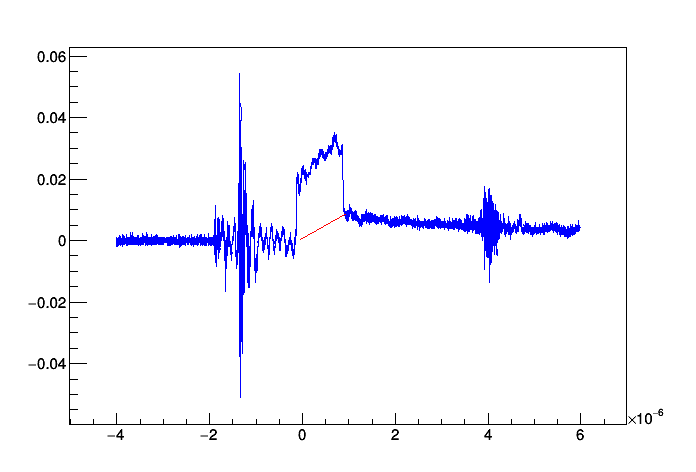
\includegraphics[width=\linewidth]{manip12_2_chambre.png} 
\caption{\label{fig:manip1_2}\footnotesize{Signal issu de la chambre pour le premier pulse de la première mesure, en haut, et du premier pulse de la dernière mesure, en bas. En rouge sont présentées les lignes de base de la contribution ionique. L'axe des abscisses est exprimé en secondes.}}
\end{center}
\end{figure}

Les résultats obtenus lors de la deuxième série de mesures montrent, figure \ref{fig:manip_largeur8}, une déformation de la réponse du PM au cours du pulse.
Cela implique d'utiliser la réponse du collimateur comme référence, celle-ci semble plus stable et cohérente.

\begin{figure}[h]
\begin{center}
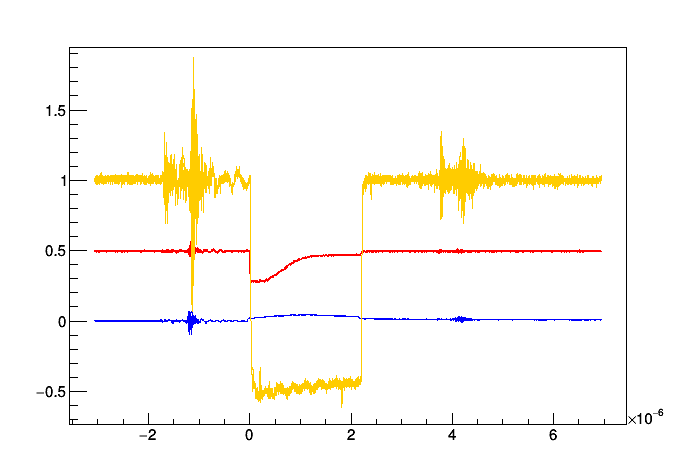
\includegraphics[width=\linewidth]{manip_largeur8-6_2.png} 
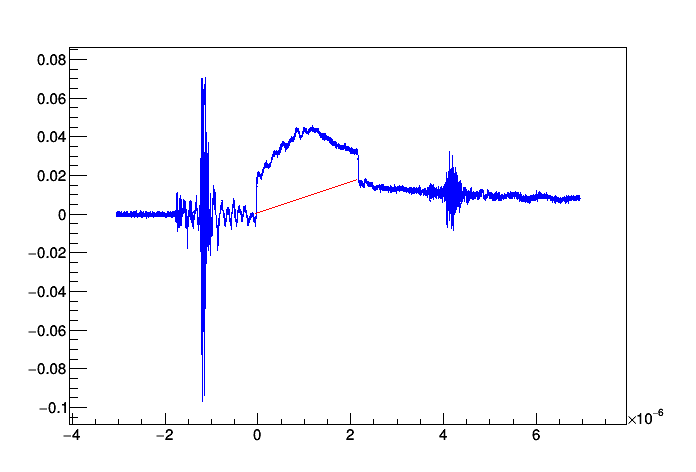
\includegraphics[width=\linewidth]{manip_largeur8-6_2_chambre.png} 
\caption{\label{fig:manip_largeur8}\footnotesize{En haut, affichage sur l'oscilloscope pour le premier pulse de la dernière mesure de la seconde série. En jaune nous avons le signal issu du collimateur, en rouge celui du PM et en bleu celui de la chambre, les deux premiers sont décalés en ordonnée pour favoriser la lecture. En bas, signal issu de la chambre pour le premier pulse de la première mesure, en haut, et du premier pulse de la dernière mesure, en bas. En rouge est présentée la ligne de base de la contribution ionique. L'axe des abscisses est exprimé en secondes.}}
\end{center}
\end{figure}

\subsection*{Réponse de la chambre}

Les résultats des mesures sont listés dans les tableaux suivants :
\begin{center}
\begin{tabular}{rl|ccc|r@{.}lr@{.}lr@{.}l}
\multicolumn{2}{c|}{Fichier}&\multicolumn{3}{c|}{Tensions (V)}&\multicolumn{6}{c}{Charges (pC)}\\
Pré.&Num.&Grille&PM&Chambre&\multicolumn{2}{r}{Chambre}&\multicolumn{2}{r}{Colli.}&\multicolumn{2}{r}{PM}\\
\hline
\hline
manip&1&100&1100&500&\hspace*{3ex}2&22&-79&99&-240&65\\
&2&120&1100&500&3&80&-174&67&-432&58\\
&3&140&1100&500&4&88&-241&53&-515&81\\
&3-1&140&1050&500&4&77&-241&13&-367&22\\
&3-2&140&1000&500&4&60&-229&76&-243&45\\
&3-3&140&950&500&4&96&-234&24&-157&96\\
&4&160&950&500&6&32&-306&55&-174&93\\
&4-1&160&900&500&6&78&-320&89&-120&99\\
&4-2&160&900&500&7&10&-319&57&-130&76\\
&5&180&900&500&8&49&-396&82&-151&52\\
&5-1&180&850&500&8&53&-400&52&-93&52\\
&6&200&850&500&10&14&-503&74&-108&60\\
&7&220&850&500&12&35&-583&04&-120&73\\
&7-1&220&850&100&6&52&-623&64&-125&77\\
&7-2&220&850&50&3&65&-638&58&-126&25\\
&7-3&220&850&200&9&93&-653&93&-127&16\\
&7-4&220&850&300&12&00&-644&10&-124&80\\
&7-5&220&850&400&13&27&-642&43&-126&67\\
&7-6&220&850&600&13&05&-635&98&-122&84\\
&7-7&220&850&700&14&25&-679&14&-131&23\\
&8&220&800&700&15&64&-710&82&-83&58\\
&9&240&800&700&17&13&-780&70&-89&35\\
&10&260&800&700&18&46&-863&61&-89&87\\
&10-1&260&750&700&18&17&-877&32&-55&80\\
&11&280&750&700&19&17&-978&57&-57&78\\
&12&300&750&700&20&66&-1066&15&-63&02\\
\hline
\end{tabular}
\end{center}

\begin{center}
\begin{tabular}{rl|cc|r@{.}lr@{.}lr@{.}l}
\multicolumn{2}{c|}{Fichier}&Largeur&Tension&\multicolumn{6}{c}{Charges (pC)}\\
Pré.&Num.&pulse ($\mu s$)&chambre (V)&\multicolumn{2}{r}{Chambre}&\multicolumn{2}{r}{Colli.}&\multicolumn{2}{r}{PM}\\
\hline
\hline
manip\_largeur&1&0.1&700&\hspace*{3ex}1&42&-27&61&-9&29\\
&1-2&0.1&700&1&59&-32&42&-10&45\\
&2&0.3&700&5&57&-273&22&-51&52\\
&3&0.5&700&10&00&-520&02&-92&81\\
&4&0.8&700&17&13&-849&67&-139&41\\
&5&1.2&700&25&95&-1301&16&-172&52\\
&6&1.4&700&29&20&-1526&36&-178&51\\
&7&1.8&700&35&55&-1985&76&-190&48\\
&8&2.2&700&41&88&-2632&20&-207&01\\
&8-1&2.2&300&25&58&-2775&47&-204&30\\
&8-3&2.2&500&35&57&-2835&56&-201&13\\
&8-4&2.2&900&49&25&-2846&60&-200&88\\
&8-5&2.2&1000&52&15&-2884&44&-201&27\\
&8-6&2.2&1200&57&75&-2937&81&-199&59\\
\hline
\end{tabular}
\end{center}

Une des premières choses que nous pouvons remarquer est que à conditions initiales de faisceau identiques, tension de grille et largeur de pulse, les réponses peuvent varier.
C'est notamment visible sur les irradiations 8 de la seconde série où le signal reçu sur le collimateur augmente sans qu'aucun de ses paramètres n'ai été changé.
Cela peut s'expliquer par la montée en température de la machine au cours du temps, ce qui augmente son efficacité.
Ça confirme qu'il est nécessaire d'exprimer la réponse de la chambre en fonction d'un paramètre sensible dans la même mesure aux conditions initiales, comme par exemple le signal du collimateur, celui du PM n'étant plus stable.

\begin{figure}[h]
\begin{center}
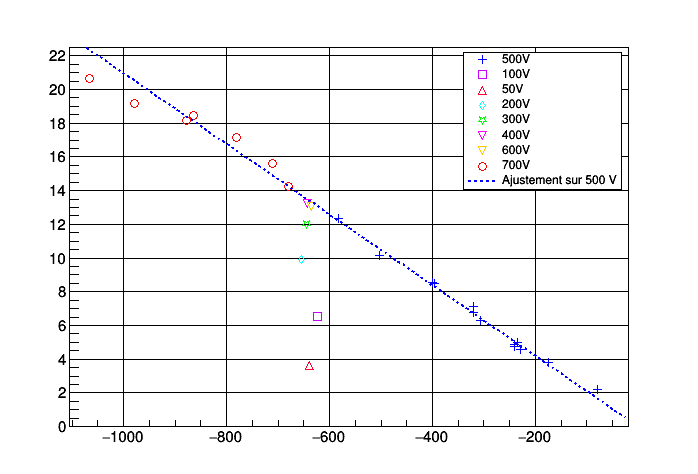
\includegraphics[width=\linewidth]{chambre_vs_colli.png} 
\caption{\label{fig:chambrevscolli}\footnotesize{Évolution de la réponse de la chambre en fonction de celle du collimateur pour différentes valeurs de tension.}}
\end{center}
\end{figure}

\begin{figure}[h]
\begin{center}
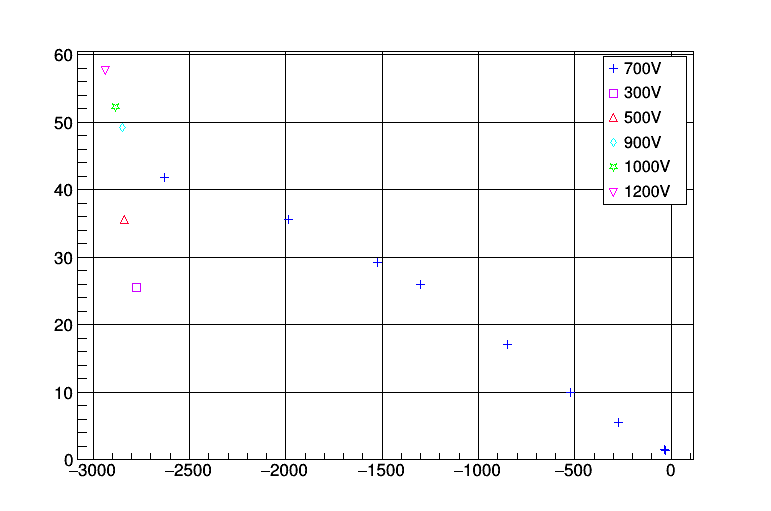
\includegraphics[width=\linewidth]{chambre_vs_colli2.png} 
\caption{\label{fig:chambrevscolli}\footnotesize{Évolution de la réponse de la chambre en fonction de celle du collimateur pour différentes valeurs de tension.}}
\end{center}
\end{figure}

%%%%%%%%%%%%%%%%%%%%%%%%%%%%%%%%%%

\end{document}

%%%%%%%%%%%%%%%%%%%%%%%%%%%%%%%%%%%%%%%%%%%%%%%%%%%%%%%%%%%%%%%%%%%%%%%%%%%%%%%%%%%%%%%%%%%%%%%%%%